\chapter{Proof of Concept}
\label{chapter_proofOfConcept}

% **************************** Define Graphics Path **************************
\ifpdf
    \graphicspath{{Chapter5/Figs/Raster/}{Chapter5/Figs/PDF/}{Chapter5/Figs/}}
\else
    \graphicspath{{Chapter5/Figs/Vector/}{Chapter5/Figs/}}
\fi

This chapter describes the steps taken to implement the algorithms presented in chapter \ref{chapter_solutions}, as well as the data gathering and pre-processing steps necessary to evaluate the algorithms, as presented in chapter \ref{chapter_evaluation}.

\section{Choice of Programming language}
While the algorithms can in theory be implemented in any programming language the programming language has, apart from personal preferences, implications on the usability of the algorithms. As a language java was chosen, due to the following reasons: There are multiple useful streaming and machine learning frameworks such as Apache Spark \cite{meng2016mllib} or Apache Flink \cite{carbone2015apache} which are also available for java. This means that the frameworks can be used in the implementation, eliminating the need to re-implement functionality like feature-based classifiers or build interfaces to other programming languages that provide such functionality (like R). Future Work can integrate the algorithms into the stream processing frameworks in order to make use of the scalability of their architecture.

\section{The implementation}

The algorithms were implemented as an eclipse Mars project using java 8. Dependencies to other projects are handled via the build-tool Maven. 

\subsection{Package Structure}

In the following the packages and subpackages are listed and briefly described.

\begin{itemize}
	\item \textbf{data} Main package for basic data representation, data gathering and basic operations on data.
	\begin{itemize}
		\item \textbf{data.crawling} contains classes for gathering raw data from the web-source
		\item \textbf{data.events} contains classes for basic event representations
		\item \textbf{data.stream} contains classes and interfaces for data streams, which can either be completely loaded into memory or read incrementally from files.
		\item \textbf{data.synthetic} contains a partial implementation of the sequence generator as suggested by Zimmermann et al. \cite{zimmermann2012generating}. This can be used to generate artificial data with specific episodes in order to test mining algorithms on it.
		\item \textbf{transformation} contains classes that implement data extraction and transformation utilities, such as extracting numerical time series from the raw data, and transforming the numerical time series to a categorical event stream.
	\end{itemize}
	\item \textbf{episode} Main package for episode patterns
	\begin{itemize}
		\item \textbf{episode.pattern} Main package for the episode patterns used in the thesis and evaluation.
		\begin{itemize}
			\item \textbf{episode.pattern.mining} contains classes implementing the general episode mining algorithm as specified in algorithm \ref{alg_generalEpisodeMining} as well as the candidate generation procedures for serial and parallel episodes as described in section \ref{sec_candidateGen}
			\item \textbf{episode.pattern.recognition} contains classes implementing the episode recognition algorithms as described in algorithms \ref{alg_SerialEpisodeDetection} and \ref{alg_ParallelEpisodeDetection}.
			\item \textbf{episode.pattern.storage} contains classes implementing episode tries for efficient storage of episodes. Also see section \ref{sec_episodeTrie} for more details on how the data structure works.
		\end{itemize}
		\item \textbf{episode.unstable\textunderscore experimental\textunderscore lossy\textunderscore counting} Package that contains experimental, less sophisticated classes to experiment with episode mining using the lossy counting algorithm. The contents of this package were not used to generate any final results as presented in chapter \ref{chapter_evaluation}.
	\end{itemize}
	\item \textbf{evaluation} contains classes that evaluate predictive models and serialize the results
	\item \textbf{experiment} main package for experiment execution and runs of the complete framework (meaning training, testing and evaluating models)
	\item \textbf{prediction} Main package for predictive models and training procedures
	\begin{itemize}
		\item \textbf{prediction.training} contains classes that extract training examples and provide utilities for model training
		\item \textbf{prediction.models} contains the model classes for all types of predictive models
	\end{itemize}		
	\item \textbf{semantics} contains all functionality to access the dbpedia \cite{auer2007dbpedia} or provide semantic knowledge in other forms.
	\item \textbf{util} contains utility classes such as standard formatters and helpful IO functionality.
\end{itemize}

\subsection{The Dependencies}
The project is realized as a maven project that has a few dependencies to other projects, these are:

\begin{itemize}
	\item \textbf{junit}: For unit testing purposes
	\item \textbf{apache-jena-libs}: Dependency to access the dbpedia via SPARQL-queries in order to use semantic knowledge.
	\item \textbf{quartz} and \textbf{quartz-jobs}: Open-source library for automatic process execution and scheduling (used in the data gathering process). Java does have built-in solutions for this, such as the \textit{ScheduledExecutorService-class} but the scheduler for processes sometimes terminated, seemingly without reason and stopped starting scheduled processes. The solution using the quartz-library does not suffer from these problems.
	\item \textbf{spark-core} and \textbf{spark-mlib}: Dependency to the apache spark library \cite{meng2016mllib}, a library for distributed big-data processing and machine learning. The library is used for its random forest implementation (which could easily be exchanged for another feature-based classifier) to use with the FBSWC algorithm.
\end{itemize}

\subsection{Basic Class Interactions}
The interactions between the classes are best explained separately for model training and evaluation. The class diagram depicted in figure \ref{fig_classDiagramTraining} shows the core classes that interact while training the models.

\begin{figure}[h]
	\centering
  	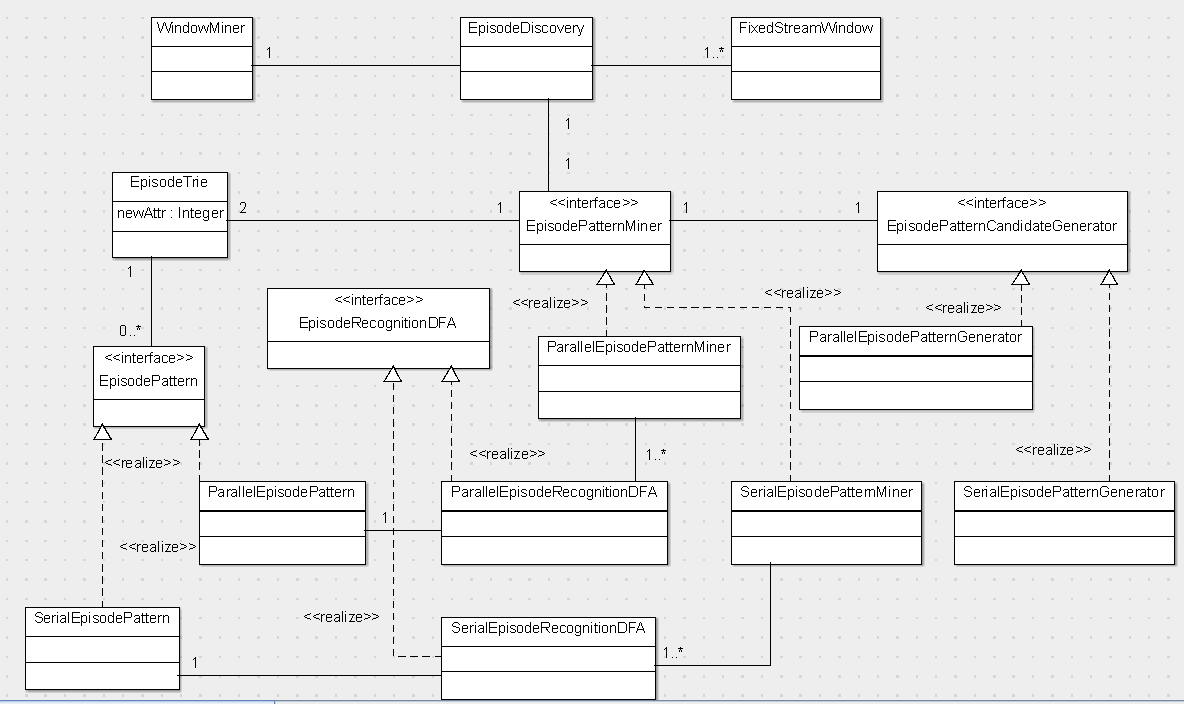
\includegraphics[width=\textwidth]{classDiagramTraining}
	\caption{Class diagram of the most important classes during the training of predictive models.}
	\label{fig_classDiagramTraining}
\end{figure}

The central class is called \textit{EpisodeDiscovery}, which makes use of the \textit{WindowMiner} to obtain the training examples, which it then provides as input to the pattern miners. In addition to the training examples the pattern miners requires

\begin{itemize}
	\item a candidate generator, meaning either a \textit{ParallelEpisodePatternGenerator} or a \textit{SerialEpisodePatternGenerator}
	\item the \textit{EpisodeTrie} as a data structure to efficiently store episodes (see section \ref{sec_episodeTrie} for a detailed explanation)
	\item a deterministic finite automaton for each episode in order to recognize it in the windows of the stream. 
\end{itemize}

Note that there are general interfaces provided, whose concrete implementations will be chosen depending on which kind of episodes are supposed to be mined (either serial or parallel). The main class interactions during the evaluation of the models is visualized in figure \ref{fig_classDiagram1}.

\begin{figure}[h]
	\centering
  	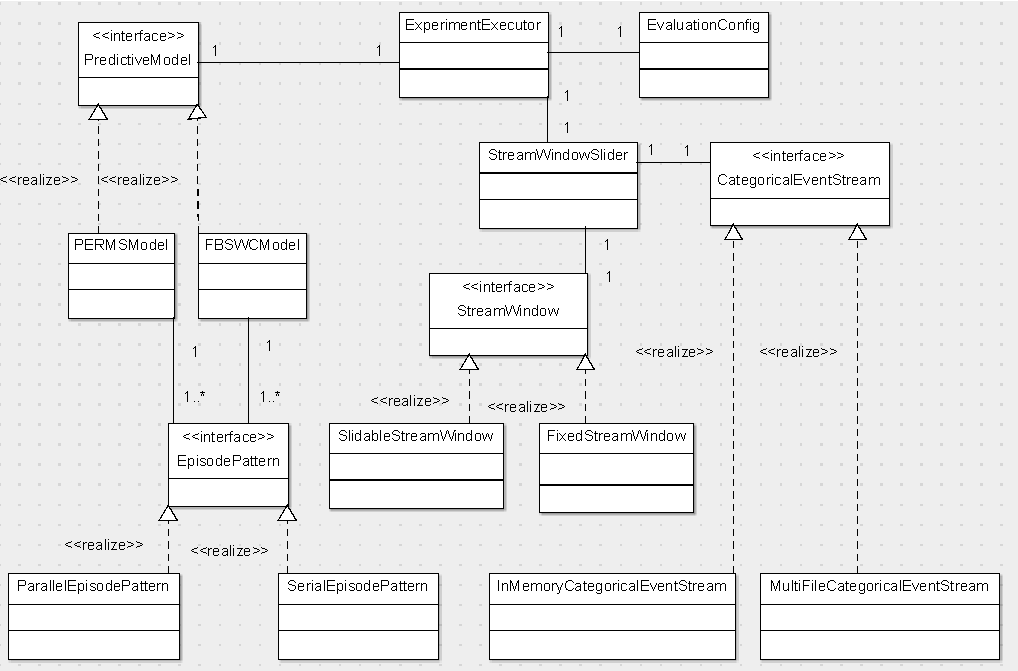
\includegraphics[width=\textwidth]{classDiagram1}
	\caption{Class diagram of the most important classes during the evaluation of predictive models.}
	\label{fig_classDiagram1}
\end{figure}

In order to evaluate constructed models, the \textit{ExperimentExecutor}-class plays the central role. It makes use of the configuration to properly initialize the models and uses the \textit{StreamWindowSlider}-class to iterate over the different stream windows of the underlying categorical event stream. Both model classes use the mined episode patterns to compute their predictions. Once again there are multiple implementations of some interfaces, allowing either for the stream to be kept in memory or be continuously read from files as well as the time windows to be fixed or slidable. 

\section{Efficient Episode Storage}
\label{sec_episodeTrie}
The naive way of storing episodes is to store each episode as a list of event types, which are sorted in alphabetical order in case of parallel episodes and according to the ordering function in case of serial episodes. This however means that each episode of length $l$ will require $\Theta(l)$ memory, which is not a lot for an individual episode but adds up when large numbers of episodes need to be kept in memory, which is the case in frequent episode mining. \\
Organizing the episodes in a trie-like data structure can greatly reduce the amount of memory needed for sets of episodes if many of these episodes have common prefixes. This idea was already put to use by Baumgarten et al. when mining sequences of sets from large sequences \cite{baumgarten2003tree}. \\
There are two types of tries: Tries for parallel episodes and tries for serial episodes. Both can be treated in exactly the same way by algorithms if the events of parallel episodes are ordered in an arbitrary but fixed order (for example alphabetically according to the event type names). In case of serial episodes the ordering is kept according to the ordering function. Figure \ref{fig_trieExample} visualizes the storage of episodes in tries. 
\begin{figure}[h]
	\centering
  	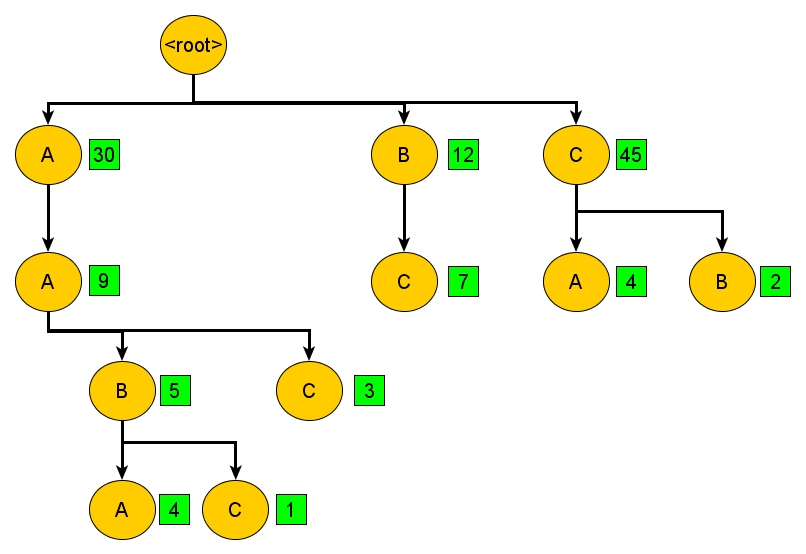
\includegraphics[width=0.75\textwidth]{trieExample}
	\caption{An example of an episode trie storing serial episodes. The yellow nodes are the nodes of the trie, each one is representing an episode. The green boxes represent the value associated with that episode, which could for example be the frequency as returned by the counting algorithms.}
	\label{fig_trieExample}
\end{figure}

The trie consists of an artificial root node, which has all episodes of length $1$ as child-nodes. Each level $i$ of the tree stores all episodes of exactly length $i$ (with the root node being level $0$). An episode is uniquely identified by a node in the tree, the whole episode can be reconstructed by walking backwards to the root of the tree. The advantage is clear: if there are episodes with the same prefix, such as $A \rightarrow A \rightarrow B \rightarrow A$ and $A \rightarrow A \rightarrow B \rightarrow C$ the prefix only needs to be stored once. Furthermore episode-frequency fulfills the a-priori criterium, which means that if an episode is present in the trie while mining frequent episodes, all its subepisodes (which are prefixes of that episode) will be present in the trie as well. Tries for parallel episodes have exactly the same structure, except that after having visited a node that is annotated with a certain event type $X$, event types that rank lower in the alphabetical order than $X$ can no longer follow.
